% !TEX root = ../main.tex
\subsection*{Phenax, God of Deception} \label{ssec::phenax}
    \subparagraph{Domains} Trickery.

    Phenax is the masked patron of lies and cheats.
    They are Heliod's ethical antithesis, governing the spheres of gambling, deception, and betrayal.
    Phenax was once a mortal who was trapped in Nyx, but they learned how to forsake their identity to prevent Erebos from detecting what they were doing.
    They crossed back over the Rivers That Ring the World wrapped in the tattered cloak of Athreos, the River Guide.
    Hidden by illusion as they were, neither Athreos nor Erebos could find Phenax and bring them back.

    % Able to play whatever role the situation calls for, Phenax is a consummate actor.
    % Their incisive wit and cunning enable them to read the desires of their marks, adjusting their approach to suit the moment.
    % In their rare moments of candor, Phenax is calm and calculating, always looking toward their next scheme.

    Phenax is a shadowy and mysterious figure.
    When appearing before mortals, they prefer the form of a willowy gat with ashen gray skin, clad in elegant robes.
    They have also been known to appear in a variety of animal forms, including the shapes of asps, mockingbirds, or rats.
    Regardless of their shape, a mask forever conceals the blank face of the first Returned.

    \begin{figure}[t]
        \centering
        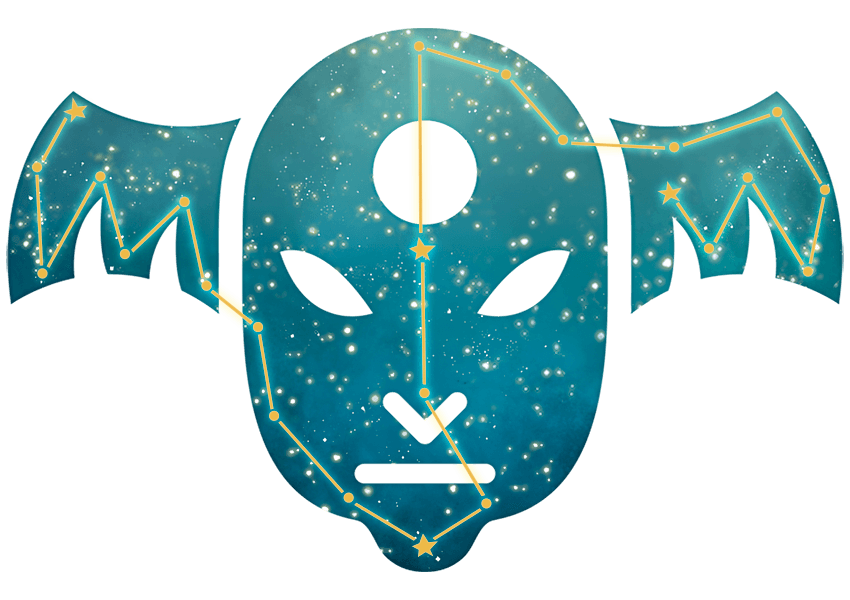
\includegraphics[width=0.47\textwidth]{02viphoger/img/10s_phenax.png}
    \end{figure}

    \subsubsection{Worshiping Phenax}
        Every lie is an homage to Phenax.
        Because their most devout followers are criminals and gamblers, their influence is keenly felt in gambling halls and dens of thieves.
        But everyone has their own reasons to stray from the truth at times, and thus, they also find small ways to seek Phenax's favor as they go about their daily lives.

        Formal services to Phenax are conducted at night, with the most sacred rituals performed on nights of the new three moons.
        Offerings are made to attract Phenax's favor, with valuables from successful robberies, parchment filled with lies, or loaded dice being thrown into deep crags or buried at crossroads.
        Such sacrifices often vanish soon after, claimed by the god or their servants.
        Devout criminals often offer Phenax stolen goods as part of their preparations for premeditated crimes.

        % Phenax is worshiped openly in the necropoleis of Asphodel and Odunos, though the Returned who are loyal to Erebos's agent, Tymaret, refuse to worship the god they're hunting.
        % Somber ceremonies are intoned to bless the golden funeral masks the Returned wear.

\subsection*{Purphoros, God of the Forge} \label{ssec::purphoros}
    \subparagraph{Domains} Forge, Knowledge.

    Purphoros is the god of the forge, the restless earth, and fire.
    They rule the raw creative force that infuses sapient minds.
    Purphoros is also the god of artisans, obsession, and the cycle of creation and destruction.

    As a forge radiates heat in the area around it, Purphoros's influence provides inspiration to mortals.
    They makes exquisitely crafted objects almost constantly, sometimes absentmindedly working while they holds conversations with the other gods, only to destroy the finished product and begin again.
    % Impulsive and mercurial, Purphoros is prone to bouts of either joyous productivity or frustrated anger.
    Purphoros often feels constrained by the limits of imagination, yearning to realize ideas that seem just out of reach.

    Purphoros's preferred form is that of a muscular treb gat whose coal-hued skin is mostly covered in mutable organic bronze.
    They might also appear in the form of a phoenix or a bull made of cooling lava, and for that reason, both of those creatures are associated with them.
    When angered, they might appear as an enormous mass of lava, a blazing fire, or a volcanic eruption.
    Mortals who see Purphoros in one of those forms seldom live to tell about it.

    \begin{figure}[b]
        \centering
        
\includegraphics[width=0.47\textwidth]{02viphoger/img/10s_purphoros.png}
    \end{figure}

    \subsubsection{Worshiping Purphoros}
        Purphoros holds dominion over everything that springs from mortal ingenuity.
        Most artisans say a small prayer to them upon beginning or completing the construction of nearly anything, from swords to fortresses to ships.

        Naturally, Purphoros is strongly associated with the forge, and nearly every smithy on Viphoger is a sort of ad hoc temple to them.
        Charms and idols of Purphoros hang from the walls in such places, intended both to inspire the artisans and protect them against accidents.
        Regardless of their professions, worshipers of Purphoros often light small fires in the god's honor, burning wooden crafts or drawings of their inventions to gain their favor.

\pagebreak

\begin{tikzpicture}[remember picture,overlay]
    \node[anchor=north, yshift=0.10cm] at (current page.north) {
\includegraphics[width=\pdfpagewidth]{02viphoger/img/10kruphix.png}};
\end{tikzpicture}

\vspace{15.0cm}

\subsection*{Thassa, God of the Sea} \label{ssec::thassa}
    \subparagraph{Domains} Knowledge, Tempest.

    Thassa is the god of the sea, aquatic creatures, and the unknown depths.
    She also holds sway over less tangible concepts such as ancient knowledge, long voyages, and gradual change.

    % Impassive and slow to anger, Thassa is secure in the knowledge that there are no mortals and few gods who can threaten her status.
    % Once her ire is aroused, however, it is as unstoppable as a cresting wave.
    % She often speaks in the future tense, referring to what tomorrow will bring.
    % She seldom laughs, and when she does, it is usually out of smugness rather than genuine mirth.

    Thassa usually appears to mortals in the form of a female tortle-like being with octopus-tentacle hair and a crown of crab legs.
    % She seldom adopts the same size as her followers, preferring to be seen from a distance as she towers over the ocean.
    When she moves close to the view of mortals, she takes many other forms, often shifting from one to another: a giant squid, an ocean storm, a school of sharks, a fog bank, or a crab, her favored animal.
    % She sometimes speaks out of the ocean itself, in droplets hissing across the surface of the waves.

    \begin{figure}[b]
        \centering
        
\includegraphics[width=0.47\textwidth]{02viphoger/img/10s_thassa.png}
    \end{figure}

    \subsubsection{Worshiping Thassa}
        Most of Thassa's dedicated worshipers are tortles.% , and the vast majority of tortles are wholly devoted to Thassa.
        Tortles spend much of their lives in Thassa's realm, with their god omnipresent.
        They weave prayers to Thassa into nearly everything they do.

        \pagebreak~
        \vspace{15.5cm}

        Among the poleis, Thassa is worshiped by those who rely on bountiful seas for sustenance or calm waters for safety.
        Sailors, fishers, and residents of Viphoger's coasts and islands all pay her at least nominal respect and sacrifice.

        % Her center of worship on land is in the coastal polis of Mephetis, where sailors and philosophers pray to her for guidance.
        % The week-long Lyokymion festival (the Feast of the Melting Swell) marks the start of the new year by celebrating the bounty of the sea.

        % Thassa's most fervent gat worshipers offer prayers at high and low tide.
        % If possible, they do so at the water's edge.
        % At low tide they walk barefoot out onto the tidal flats, relishing the touch of Thassa's seabed.
